\documentclass[a4paper]{article} %format de la feuille + type de document https://en.wikibooks.org/wiki/LaTeX/Document_Structure#Document_classes
%packages nécessaire pour nos besoins
\usepackage[utf8]{inputenc}
\usepackage[T1]{fontenc}
\usepackage[english,french]{babel}
\usepackage{amsmath}
\usepackage{amssymb,amsfonts,textcomp}
\usepackage{color}
\usepackage{array}
\usepackage{hhline}
\usepackage{hyperref}
\usepackage[pdftex]{graphicx}
\usepackage{sectsty}
\usepackage{tcolorbox}
\usepackage{textcomp}
\usepackage{courier}
\usepackage[font={small,it}]{caption}
\usepackage{float}
\usepackage{graphicx}
\usepackage{caption}
\usepackage{tabularx}
\usepackage{multirow}% http://ctan.org/pkg/multirow
\usepackage{tikz}
\usepackage[top=15mm,bottom=20mm,right=50mm,left=50mm]{geometry} 
\usepackage[export]{adjustbox}


%Définition des couleurs
\definecolor{havelockBlue}{rgb}{0.004, 0.42, 0.73}
\definecolor{Monokaimagenta}{rgb}{0.86,0.08,0.24}

%utilisation de la couleur définie avant
%toutes les sections auront cette couleur
\sectionfont{\color{havelockBlue}}
%\subsectionfont{\color{havelockBlue}}
%début du document
\begin{document}

\renewcommand{\labelitemi}{$\bullet$}
\renewcommand{\labelitemii}{$\cdot$}
\renewcommand{\labelitemiii}{$\diamond$}
\renewcommand{\labelitemiv}{$\ast$}

%début d'un titre
\begin{titlepage}
            %centre les éléments
	\centering
	
	{\scshape\LARGE \color{Monokaimagenta} Laboratoire \\  \par}
	
	%espace vertical de 1 mms
	\vspace{1cm}
	
	{\Large\itshape Sven Rouvinez \& Johanna Melly\par}
	
	%http://www.personal.ceu.hu/tex/spacebox.htm
	\vfill
	Professeur\par
	%met le texte en gras 
	\textbf{Carlos Andrés Pena} \par% ajoute une ligne 
	\vspace{1cm}
	Assistant\par
	\textbf{Gaëtan Matthey}
	
	\vfill

            %affiche la date actuelle
	{\large \today\par}
	
%fin de la page de titre
\end{titlepage}

\section{Objectifs du laboratoire}
Ce laboratoire consistait en la réalisation d'un décodeur, qui comprenait aussi une partie gérant les instruction MOV et ADD. Son bon fonctionnement devait être testé à l'aide du main fourni dans le workspace du laboratoire.

\section{Blocs Logisim}
Nous avons décidé de séparer les blocs afin de permettre une meilleure modularité et abstraction du système DECODE.\\
\paragraph{Résumé}
\begin{itemize}
    \item     MOV\_INST détecte une instruction \textbf{MOV}
    \item     ADD\_INST détecte une instruction \textbf{ADD}
    \item     REGISTER\_16BITS banque de registres
    \item     DECODE Décode les instructions \textbf{MOV} et \textbf{ADD} et les transmet à la banque de registre
    \item     main bloc principal, avec la mémoire contenant les instructions, et le \textbf{DECODE}
\end{itemize}
\subsection{MOV\_INST}

\begin{figure}[H]
    \centering
    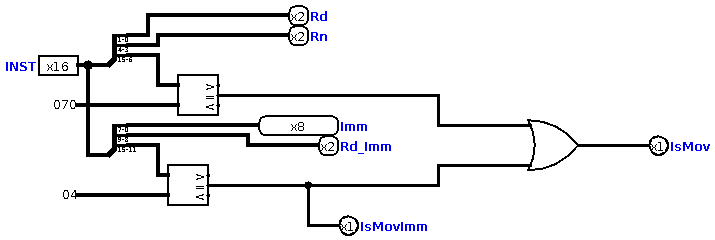
\includegraphics[width=.8\textwidth]{src/MOV_INST.png}
    \caption{Instruction MOV}
    \label{mov_img}
\end{figure}
\paragraph{Définition des entrées:}
\begin{itemize}
    \item     INST: code complet
    \item     0x70: code recherché pour un MOV avec valeur non immédiate
    \item     0x04: code recherché pour un MOV avec valeur immédiate
\end{itemize}

\paragraph{Définition des sorties:}
\begin{itemize}
    \item     Rd: registre destination
    \item     Rn: registre source
    \item     isMOV: s'active si les bits de 15 à 9 sont égaux à $0001110$ (0x70) ou à $0000010$ (0x04).
    \item     Imm: valeur immédiate
    \item     Rd\_Imm: registre destination pour MOV avec valeur immédiate
    \item     isMovimm: s'active si on a un MOV avec valeur immédiate

\end{itemize}

\medskip

Ce bloc permet de détecter si une instruction \textbf{MOV} est trouvée, grâce au comparateur, dans le code de sortie de la ROM, cette instruction va charger la valeur du registre source (Rn) dans le registre destination (Rd).\\
Elle se caractérise par le code ci-dessous : 
\\
\begin{tabular}{|ccccccc|ccc|ccc|ccc|}
    \hline
    \multicolumn{7}{|c|}{Code ARM}  & \multicolumn{3}{|c|}{Opcode} & \multicolumn{3}{|c|}{Rn} & \multicolumn{3}{|c|}{Rd}\\
    \hline
    15 & 14 & 13 & 12 & 11 & 10 & 9 & 8 & 7 & 6                    & 5 & 4 & 3                & 2 & 1 & 0 \\
    \hline
    0  & 0  & 0  & 1  & 1  & 1  & 0 & 0 & 0 & 0                    & 1 & 0 & 0                & 1 & 0 & 1 \\
    \hline     
    \end{tabular}
\\

\begin{itemize}
    \item     Code ARM : instruction ARM à effectuer
    \item     Opcode : instruction à effectuer par l'ALU
    \item     Rn : registre source
    \item     Rd : registre destination
\end{itemize}

\medskip
Nous avons donc deux code ARM différents, selon la valeur donnée pour RD, qui peut être une valeur imméiate (en héxadécimal). Ainsi, dans ce bloc, on a les sorties correspondant au registres et valeurs concernées, et on peut vérifier le type de donnée grâce à la sortie \textbf{isMovImm} qui va indiquer le type de donnée. La sortie \textbf{isMOV} va être activée, indépendamment de s'il s'agit d'une valeur immédiate ou non, puisqu'elle indique uniquement s'il y a eu une instruction MOV.


\subsection{ADD\_INST} \label{addinst}
\begin{figure}[H]
    \centering
    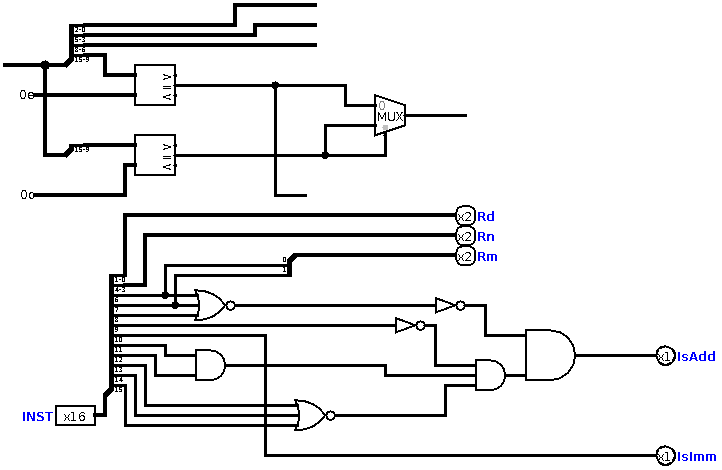
\includegraphics[width=.8\textwidth]{src/ADD_INST.png}
    \caption{Instruction ADD}
    \label{add_img}
\end{figure}

\paragraph{Définition des entrées:}
\begin{itemize}
    \item     INST: code complet
\end{itemize}

\paragraph{Définition des sorties:}
\begin{itemize}
    \item     Rd: registre destination
    \item     Rn: registre source 2
    \item     Rm: registre source 1
    \item     isAdd: s'active si l'instruction ADD est détectée
    \item     isImm: s'active s'il y a une valeur immédiate
\end{itemize}
\medskip 

L'instruction ADD se présente comme suit:

\begin{tabular}{|ccccccc|ccc|ccc|ccc|}
    \hline
    \multicolumn{7}{|c|}{Code ARM}  & \multicolumn{3}{|c|}{Opcode} & \multicolumn{3}{|c|}{Rn} & \multicolumn{3}{|c|}{Rd}\\
    \hline
    15 & 14 & 13 & 12 & 11 & 10  & 9 & 8   & 7   & 6                 & 5 & 4 & 3                & 2   & 1   & 0 \\
    \hline
    0  & 0  & 0  & 1  & 1  & 1/0 & 0 & 1/0 & 1/0 & 1/0               & 1/0 & 1/0 & 1/0                & 1/0 & 1/0 & 1/0 \\
    \hline     
    \end{tabular}
     \medskip \\
    Le circuit ADD fonctionne ce cette manière: les bits 15-13 doivent être à 0, et passent donc dans une porte NOR. Si la sortie est à 1, c'est que les 3 bits sont à zéro (ce que l'on cherche ici). Les bits 12-11, quant à eux, doivent être à 1. Ils passent donc dans une porte AND pour vérifier que ce soit le cas. Le bit 10 indique s'il d'agit d'une valeur immédiate (1) ou non (0). Le bit 9 insique s'il agit d'un ADD (0) ou d'un SUB (1), ainsi, il est suivi d'un NOT pour obtenir un 1 s'il s'agit bien d'une instruction ADD. Les bits 8-6 correspondent à l'offset, et les bits 7-6 au registre source 1 s'il n'y a pas de valeur immédiate. Les bits 4-3 correspondent au registre source 2, et les bits 1-0 au registre destination.
    La sortie est précédé d'un porte AND qui vérifie que les critères permettant de reconnaître qu'il s'agit bien d'une instruction ADD.
    
    
\subsection{REGISTER\_16BITS} \label{regi16}
\begin{figure}[H]
    \centering
    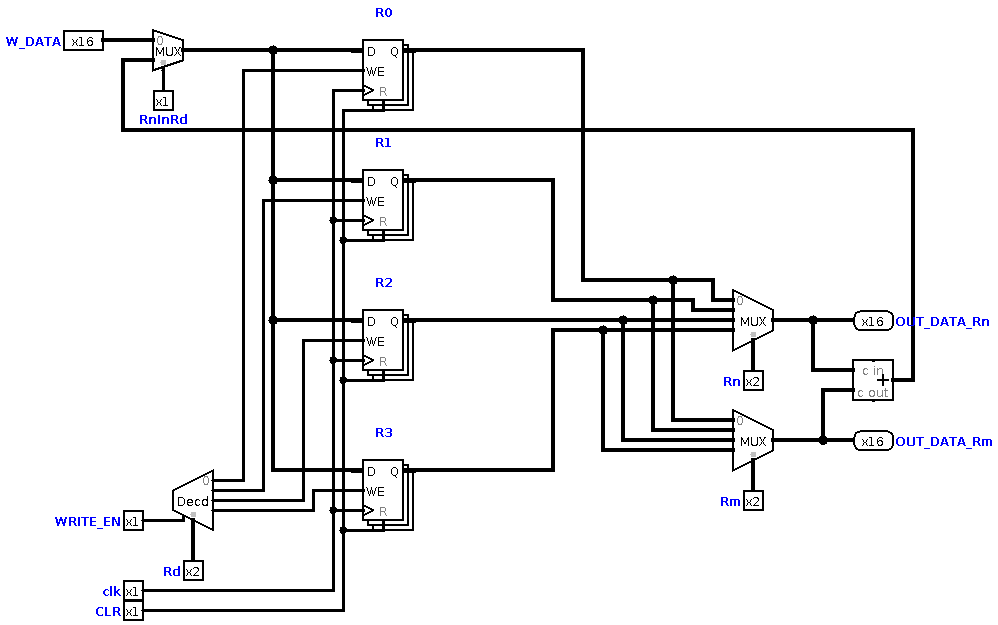
\includegraphics[width=.8\textwidth]{src/REGISTERS_16BITS.png}
    \caption{Banque de registres}
    \label{regi16_img}
\end{figure}



\paragraph{Définition des entrées:}
\begin{itemize}
    \item     W\_DATA: contient les données à entrer
    \item     WRITE\_EN: active l'écriture
    \item     clk: horloge
    \item     CRL: reset
    \item     Rd: registre destination
    \item     RnInRd: est actif si on n'a pas de valeur immédiate
\end{itemize}
\paragraph{Définition des sorties:}
\begin{itemize}
    \item Rn: registre source 2
    \item Rm: registre source 1
    \item OUT\_DATA\_Rn: sortie correspondant au registre 2
    \item OUT\_DATA\_Rm: sortie correspondant au registre 1
\end{itemize}
\medskip
Ce bloc est composé d'une partie permettant de choisir le type de donnée, une choisissant le registre dans lequel inscrire les données, et une permettant la sortie des adresses, selon le registre.
Ainsi, les données sont reçue en entré \textbf{W\_DATA}, elle-même en entrée dans un MUX qui détermine s'il fait envoyer la valeur immédiate aux registres, ou une valeur calculée. Si l'entrée \textbf{WRITE\_EN} est active, alors le decode va permettre l'écriture dans un registre choisi (grâce à \textbf{Rd}) des données.
En sortie, deux MUX permettent de choisir le registre dont on veut les données en sortie.



\subsection{DECODE}
\begin{figure}[H]
    \centering
    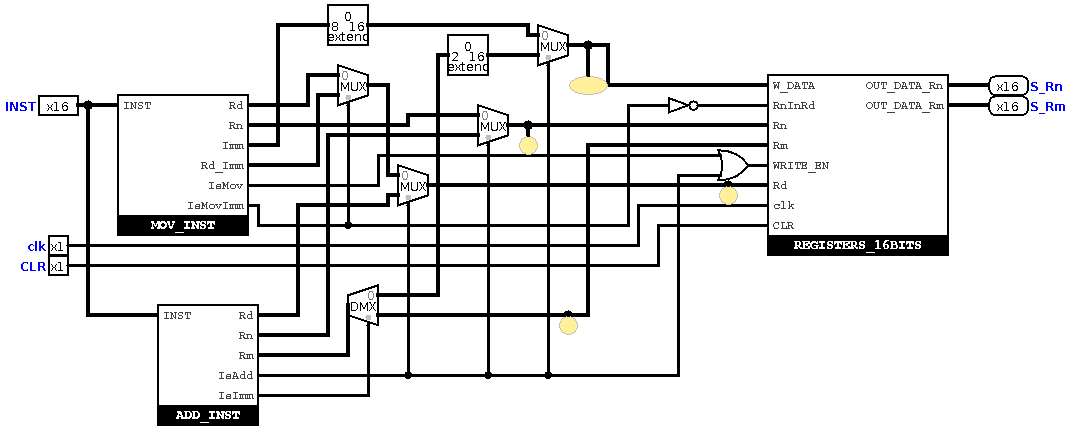
\includegraphics[width=1\textwidth]{src/DECODE.png}
    \caption{Decode}
    \label{decode_img}
\end{figure}

\paragraph{Définition des entrées:}
\begin{itemize}
    \item     INST: instruction à effectuer
    \item     clk: horloge
    \item     CLR: reset
\end{itemize}

\paragraph{Définition des sorties:}
\begin{itemize}
    \item     S\_Rn: Registre source 2
    \item     S\_Rm: Registre source 1
\end{itemize}
\medskip
Les sorties des blocs \textbf{MOV\_INST} et \textbf{ADD\_INST} étant toutes reliées à des entrées du bloc \textbf{REGISTERS\_16BITS}, le \textbf{DECODE} sera expliqué en décrivant les liens par rapport aux différentes entrées du bloc \textbf{REGISTER\_16BITS}. \medskip \\
\textbf{W\_DATA}: cette entrée est reliée aux sorties \textbf{Imm} du \textbf{MOV\_INST} et \textbf{Rm} du bloc \textbf{ADD\_INST}. Elle va prendre les valeurs immédiate en sortie de MOV et ADD, selon l'instruction donnée. Imm correpond à la valeur immédiate de l'instruction MOV et est sur 8 bit, elle passe donc dans un EXTEND qui permet de l'étendre à 16 bits. Rm est le registre source 1 de l'ADD. Il peut être sous forme de valeur immédiate ou non, c'est pourquoi il passe tout d'abord dans un démultiplexer, donc la sortie 0 correspond à une valeur immédiate, et va être reliée à un EXTEND qui va étendre la valeur sur 16 bit. Les deux valeurs immédiates (de MOV et de ADD) sur 16 bits sont reliées à un multiplexer. Ce dernier va envoyer la valeur en sortie de MOV si IsAdd (qui indique s'il y a une instruction ADD) est à 0, et la valeur en sortie de ADD si IsAdd est à 1. \medskip \\
\textbf{RnInRd}: prend en entrée un NOT IsMovImm, qui indique que la valeur de l'instruction MOV n'est pas immédiate.\medskip \\
\textbf{Rn}: prend en entrée le registre source 1, soit en sortie de \textbf{ADD\_INST} soit en sortie de \textbf{MOV\_INST}. Le bloc à choisir est déterminé par un multiplexer, qui est à 1 si IsAdd est activé.\medskip \\
\textbf{Rm}: prend en entrée le registre source en sortie de \textbf{ADD\_INST}, si celui-ci n'est pas une valeur immédiate (vérifié par un multiplexer).
\medskip \\
\textbf{RmDataZero}: est activé si on a une instruction MOV, puisqu'elle ne possède qu'un registre source. Ainsi, on relie la sortie IsMov, qui indique s'il s'agit a bien une instruction MOV.
\medskip \\
\textbf{WRITE\_EN}: s'active si on a une instruction MOV ou ADD. Ainsi, est relié à une porte OR qui prend en entrée IsAdd et IsMov.
\medskip \\
\textbf{Rd}: l'entrée Rd du REGISTER prend en entrée la sortie Rd du bloc \textbf{ADD\_INST} ou du bloc \textbf{MOV\_INST}, selon l'instruction voulue (choisie par un multiplexer dont la valeur est déterminée par IsAdd). Le registre destination du bloc \textbf{MOV\_INST} peut être une valeur immédiate ou non, raison pour laquelle il y a un multiplexer prenant en entrée les valeurs immédiate (qu'il prend en compte à 1) et non immédiate de ce bloc (qu'il prend en compte à 0), et qui passe à 1 lorsque IsMovImm (qui indique si la valeur est immédiate) est activée.
\medskip \\
Les deux dernière entrées du bloc (clk et CLR) sont simplement l'horloge et le reset.



\subsection{main}
\begin{figure}[H]
    \centering
    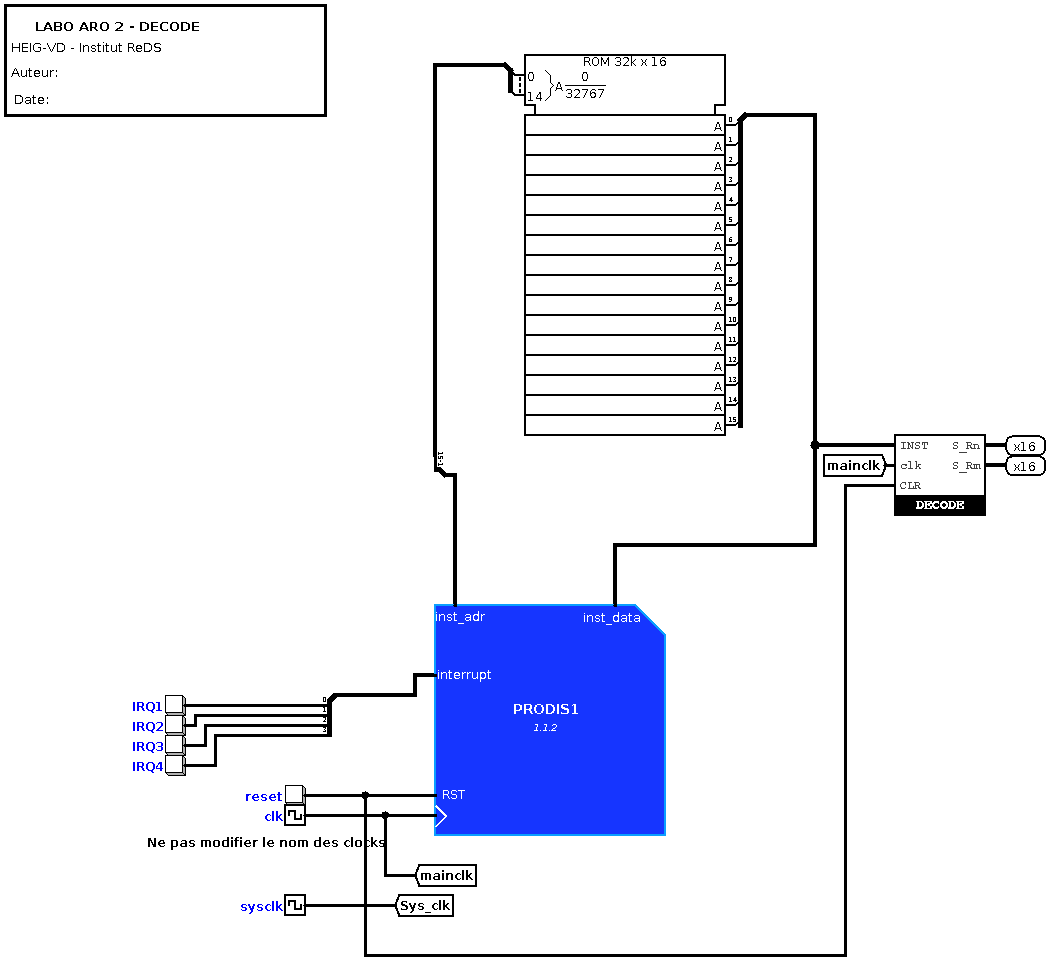
\includegraphics[width=1\textwidth]{src/main.png}
    \caption{Main program}
    \label{main_img}
\end{figure}

Le main program  nous a permis de contrôler le bon fonctionnement de notre DECODE. Nous avions en instruction:

\begin{tabular}{|c|c|c|c|}
    
    \hline
    INST & Rd & Rn  & Rm  \\
    \hline
    MOV  & r1 & \#2  &    \\
    \hline
    MOV  & r1 & \#2  &    \\
    \hline
    ADD  & r2 & r1   & r3 \\
    \hline
    MOV  & r1 & \#12 &    \\
    \hline
    ADD  & r0 & r1   & r2 \\
    \hline
    MOV  & r3 & r0   &    \\
    \hline
\end{tabular}
    
    




\section{Conclusion}
Dans ce laboratoire, nous avons pu mettre en pratique la théorie vue en classe, qui peut parfois être un peu floue jusqu'à avoir un exemple concret. Nous avons appris à manipuler des adresses de mémoire et des instructions, compris le fonctionnement de ces dernières et la façon dont elles étaient segmentées, chaque portion de bits contenant une information qui permet d'effectuer les bonnes opérations aux bons endroits. \\
Nous avons remarqué que la séparation des gros circuits en plus petits circuits permettait une bien meilleure lisibilité, ainsi nous avons séparé l'entier du circuit.
\section{Annexes}

\end{document}